\documentclass{oblivoir}
%%%Default packages
\usepackage{amsmath,amssymb,amsthm,kotex,tabu,graphicx,pifont}
\usepackage{../kswrapfig}

\usepackage{gensymb} %\degree

%%%More packages
%\usepackage{caption,subcaption}
%\usepackage[perpage]{footmisc}
%
\usepackage[skipabove=10pt,innertopmargin=10pt,nobreak=true]{mdframed}

\usepackage[inline]{enumitem}
\setlist[enumerate,1]{label=(\arabic*)}
\setlist[enumerate,2]{label=(\alph*)}

\usepackage{multicol}
\setlength{\columnsep}{30pt}
\setlength{\columnseprule}{1pt}
%
%\usepackage{forest}
%\usetikzlibrary{shapes.geometric,arrows.meta,calc}
%
%%%defi theo exam prob rema proo
%이 환경들 아래에 문단을 쓸 경우 살짝 들여쓰기가 되므로 \hspace{-.7em}가 필요할 수 있다.

\newcounter{num}
\newcommand{\defi}[1]
{\noindent\refstepcounter{num}\textbf{정의 \arabic{num})} #1\par\noindent}
\newcommand{\theo}[1]
{\noindent\refstepcounter{num}\textbf{정리 \arabic{num})} #1\par\noindent}
\newcommand{\revi}[1]
{\noindent\refstepcounter{num}\textbf{복습 \arabic{num})} #1\par\noindent}
\newcommand{\exam}[1]
{\bigskip\bigskip\noindent\refstepcounter{num}\textbf{예시 \arabic{num})} #1\par\noindent}
\newcommand{\prob}[1]
{\bigskip\bigskip\noindent\refstepcounter{num}\textbf{문제 \arabic{num})} #1\par\noindent}
\newcommand{\rema}[1]
{\bigskip\bigskip\noindent\refstepcounter{num}\textbf{참고 \arabic{num})} #1\par\noindent}
\newcommand{\proo}
{\bigskip\noindent\textsf{증명)}}

\newenvironment{talign}
 {\let\displaystyle\textstyle\align}
 {\endalign}
\newenvironment{talign*}
 {\let\displaystyle\textstyle\csname align*\endcsname}
 {\endalign}
%
%%%Commands

\newcommand{\procedure}[1]{\begin{mdframed}\vspace{#1\textheight}\end{mdframed}}

\newcommand\an[1]{\par\bigskip\noindent\textbf{문제 \ref{#1})}\par\noindent}

\newcommand\ann[2]{\par\bigskip\noindent\textbf{문제 \ref{#1})}\:\:#2\par\medskip\noindent}

\newcommand\ans[1]{\begin{flushright}\textbf{답 : }#1\end{flushright}}

\newcommand\anssec[1]{\bigskip\bigskip\noindent{\large\bfseries#1}}

\newcommand{\pb}[1]%\Phantom + fBox
{\fbox{\phantom{\ensuremath{#1}}}}

\newcommand\ba{\,|\,}

\newcommand\ovv[1]{\ensuremath{\overline{#1}}}
\newcommand\ov[2]{\ensuremath{\overline{#1#2}}}
%
%%%% Settings
%\let\oldsection\section
%
%\renewcommand\section{\clearpage\oldsection}
%
%\let\emph\textsf
%
%\renewcommand{\arraystretch}{1.5}
%
%%%% Footnotes
%\makeatletter
%\def\@fnsymbol#1{\ensuremath{\ifcase#1\or
%*\or **\or ***\or
%\star\or\star\star\or\star\star\star\or
%\dagger\or\dagger\dagger\or\dagger\dagger\dagger
%\else\@ctrerr\fi}}
%
%\renewcommand{\thefootnote}{\fnsymbol{footnote}}
%\makeatother
%
%\makeatletter
%\AtBeginEnvironment{mdframed}{%
%\def\@fnsymbol#1{\ensuremath{\ifcase#1\or
%*\or **\or ***\or
%\star\or\star\star\or\star\star\star\or
%\dagger\or\dagger\dagger\or\dagger\dagger\dagger
%\else\@ctrerr\fi}}%
%}   
%\renewcommand\thempfootnote{\fnsymbol{mpfootnote}}
%\makeatother
%
%%% 객관식 선지
\newcommand\one{\ding{172}}
\newcommand\two{\ding{173}}
\newcommand\three{\ding{174}}
\newcommand\four{\ding{175}}
\newcommand\five{\ding{176}}
\usepackage{tabto,pifont}
%\TabPositions{0.2\textwidth,0.4\textwidth,0.6\textwidth,0.8\textwidth}

\newcommand\taba[5]{\par\noindent
\one\:{#1}
\tabto{0.2\textwidth}\two\:\:{#2}
\tabto{0.4\textwidth}\three\:\:{#3}
\tabto{0.6\textwidth}\four\:\:{#4}
\tabto{0.8\textwidth}\five\:\:{#5}}

\newcommand\tabb[5]{\par\noindent
\one\:{#1}
\tabto{0.33\textwidth}\two\:\:{#2}
\tabto{0.67\textwidth}\three\:\:{#3}\medskip\par\noindent
\four\:\:{#4}
\tabto{0.33\textwidth}\five\:\:{#5}}

\newcommand\tabc[5]{\par\noindent
\one\:{#1}
\tabto{0.5\textwidth}\two\:\:{#2}\medskip\par\noindent
\three\:\:{#3}
\tabto{0.5\textwidth}\four\:\:{#4}\medskip\par\noindent
\five\:\:{#5}}

\newcommand\tabd[5]{\par\noindent
\one\:{#1}\medskip\par\noindent
\two\:\:{#2}\medskip\par\noindent
\three\:\:{#3}\medskip\par\noindent
\four\:\:{#4}\medskip\par\noindent
\five\:\:{#5}}
%
%%%% fonts
%
%\usepackage{fontspec, xunicode, xltxtra}
%\setmainfont[]{은 바탕}
%\setsansfont[]{은 돋움}
%\setmonofont[]{은 바탕}
%\XeTeXlinebreaklocale "ko"
\usepackage{movie15}

%%% Title
\title{미적분 1 : 03 미분계수와 도함수}
\date{\today}
\author{}

\begin{document}
\maketitle

\tableofcontents
\clearpage

%%
\section{복습}
%
\exam{직선의 기울기}
\begin{enumerate}
\item
직선 \(y=2x+1\)의 기울기는 \(2\)이고 \(y\)절편은 \(1\)이다.
이때 \emph{기울기}란 직선이 기울어진 정도로서
\[\text{기울기}=\frac{x\text{의 값의 증가량}}{y\text{의 값의 증가량}}\]
으로 계산한다.
이때 기울기는 항상 일정한 값 \(2\)를 가진다는 것을 관찰할 수 있다.
\[\text{기울기}=\frac{\Delta y}{\Delta x}=\frac21=\frac42.\]
\item
만약 \(x\)의 값이 증가할 때 \(y\)의 값이 감소한다면, \(y\)의 값의 증가량은 음수로 나타낸다.
예를 들어, 직선 \(y=-x+4\)의 기울기는 \(-1\)이다.
\[\text{기울기}=\frac{\Delta y}{\Delta x}=\frac{-1}1=\frac{-2}2.\]
\end{enumerate}
\begin{center}
\begin{tabular}{cc}
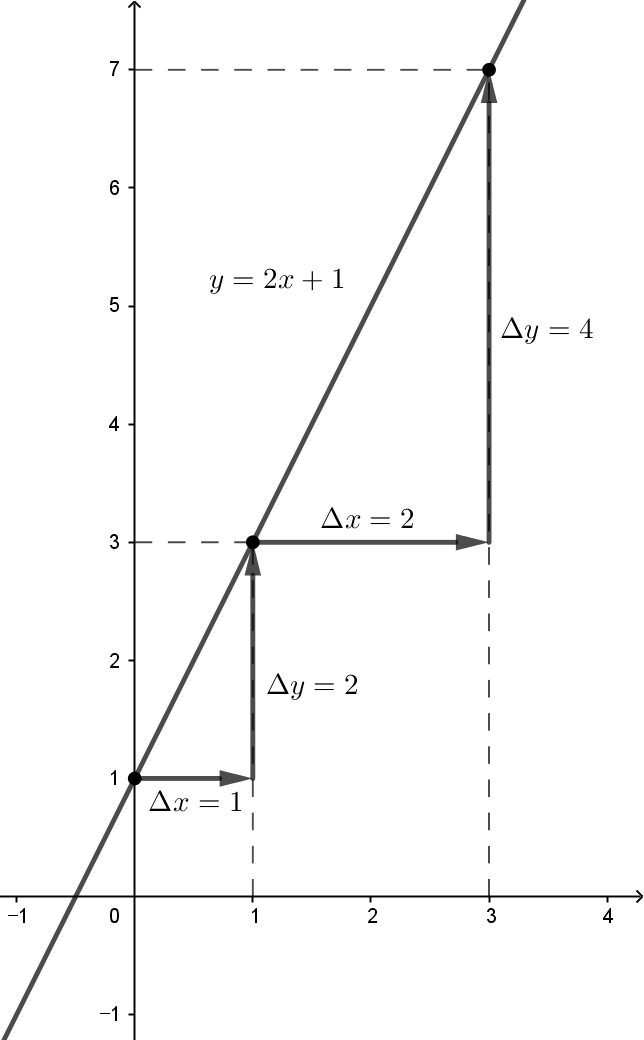
\includegraphics[width=.48\textwidth]{slope1}
&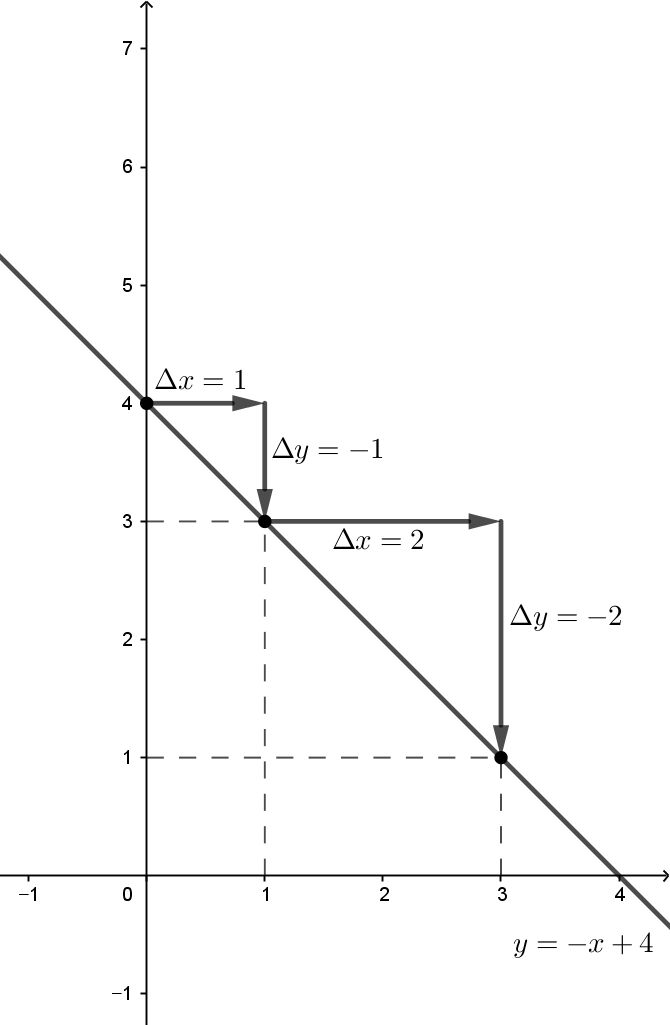
\includegraphics[width=.48\textwidth]{slope2}
\end{tabular}
\end{center}

%
\prob{다음 직선들에 대하여 기울기를 계산하여라.}
\begin{center}
\begin{tabular}{cc}
(1) \(y=-3x+1\)
&(2) \(y=\frac12x+2\)\\
\includegraphics[width=.35\textwidth]{55}
&\includegraphics[width=.35\textwidth]{55}
\end{tabular}
\end{center}

%
\exam{이차함수 \(y=x^2+2\) 위의 한 점 \((1,3)\)에서의 접선의 방정식을 구하여라.}

\begin{mdframed}
접선의 기울기를 \(m\)이라고 두면, 이 접선의 방정식을
\[y=m(x-1)+3\]
이라고 둘 수 있다.

이때, 포물선과 직선이 접하기 위해서는 교점의 개수가 한 개여야 한다.
따라서 연립방정식
\[\begin{cases}
y&=x^2+2\\
y&=m(x-1)+3
\end{cases}\]
은 단 하나의 근을 가져야 한다.
즉 이차방정식
\begin{gather*}
x^2+2=mx-m+3\\
x^2-mx+m-1=0
\end{gather*}
의 판별식의 값이 0이어야 한다;
\[D=(-m)^2-4\cdot1\cdot(m-1)=m^2-4m+4=0\]
따라서 \(m=2\)이고, 접선의 방정식은 \(y=2x+1\)이다.
\end{mdframed}
\begin{center}
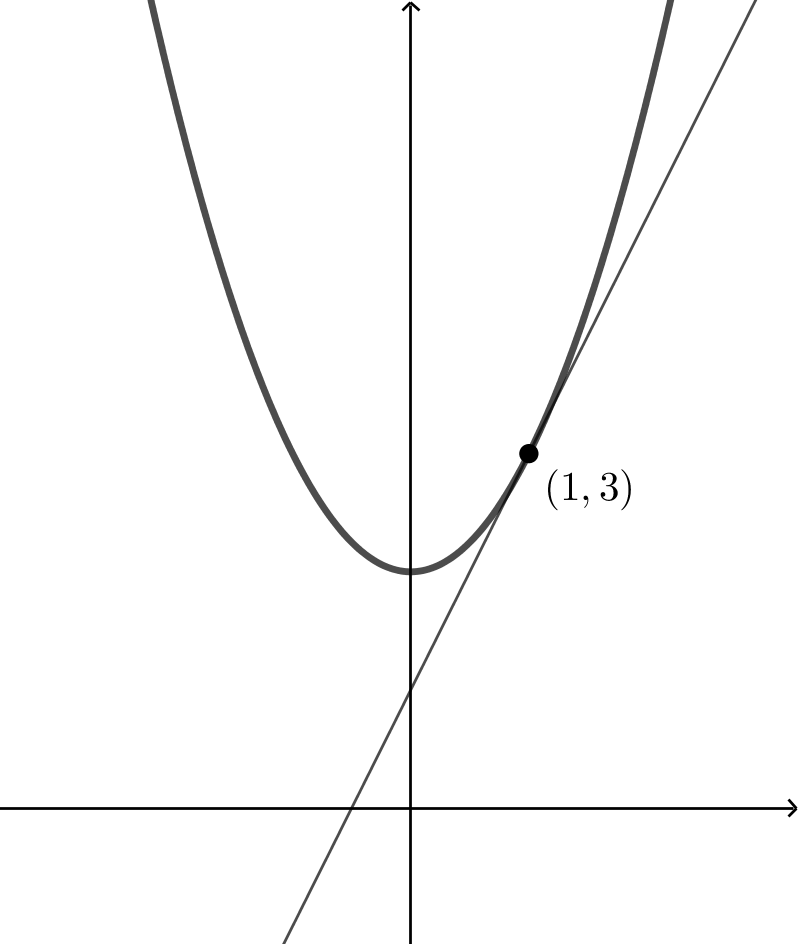
\includegraphics[width=0.4\textwidth]{tangent}
\end{center}

%
\prob{이차함수 \(y=-x^2+6x-4\) 위의 한 점 \((1,1)\)에서의 접선의 방정식을 구하여라.}
\bigskip

\clearpage
%%
\section{평균변화율}
함수 \(y=f(x)\)에서 \(x\)의 값이 \(a\)에서 \(b\)까지 변할 때, 함숫값 \(y\)는 \(f(a)\)에서 \(f(b)\)까지 변한다.
이때 \(x\)의 변화량인 \(b-a\)를 \(x\)의 \emph{증분}, \(y\)의 변화량인 \(f(b)-f(a)\)를 \(y\)의 증분이라고 부르며 각각 \(\Delta x\), \(\Delta y\)라고 표시한다.
\begin{align*}
\Delta x &= b-a\\
\Delta y &= f(b)-f(a)
\end{align*}
이때, \emph{평균변화율}이란 \(\Delta y\)를 \(\Delta x\)로 나눈 값을 말한다;
\[\frac{\Delta y}{\Delta x}=\frac{f(b)-f(a)}{b-a}=\frac{f(a+\Delta x)-f(a)}{\Delta x}.\]

\begin{center}
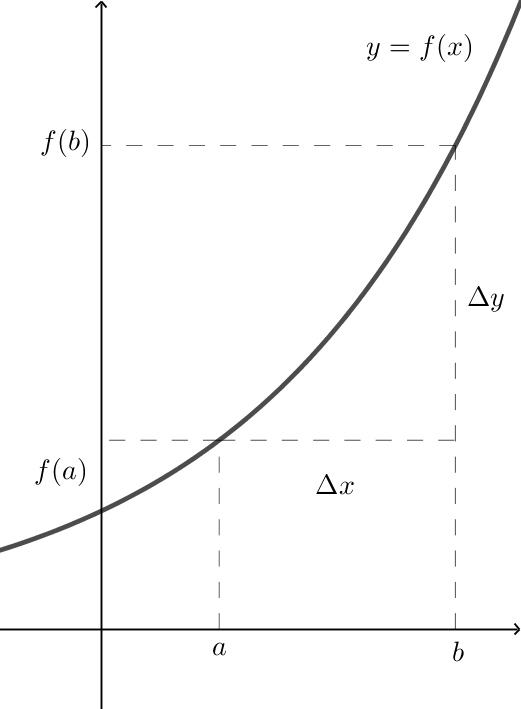
\includegraphics[width=.4\textwidth]{average_rate}
\end{center}

\vspace{-15pt}
%
\exam{다음 함수들에 대하여 \(x=1\)에서 \(x=3\)까지의 평균변화율을 구하여라.}
\begin{tabularx}{\textwidth}{XX}
(1) \(f(x)=2x^2+1\)
&
(2) \(g(x)=2x+3\)
\end{tabularx}
\vspace{-15pt}
\begin{mdframed}
\vspace{-20pt}
\begin{align*}
(1)&\:\text{평균변화율}=\frac{f(3)-f(1)}{3-1}=\frac{19-3}2=8\\
(2)&\:\text{평균변화율}=\frac{g(3)-g(1)}{3-1}=\frac{9-5}2=2
\end{align*}
\end{mdframed}

%
\prob{다음 함수들에 대하여 \(x=-1\)에서 \(x=3\)까지의 평균변화율을 구하여라.}
\begin{tabularx}{\textwidth}{XXX}
(1) \(f(x)=-\frac23x+1\)
&
(2) \(g(x)=x^2\)
&
(3) \(h(x)=|2x-2|+1\)
\end{tabularx}

%%
\section{순간변화율(미분계수)}

\end{document}